\documentclass{standalone}
\usepackage{tikz}
\usetikzlibrary{calc}

%% Document
\begin{document}

	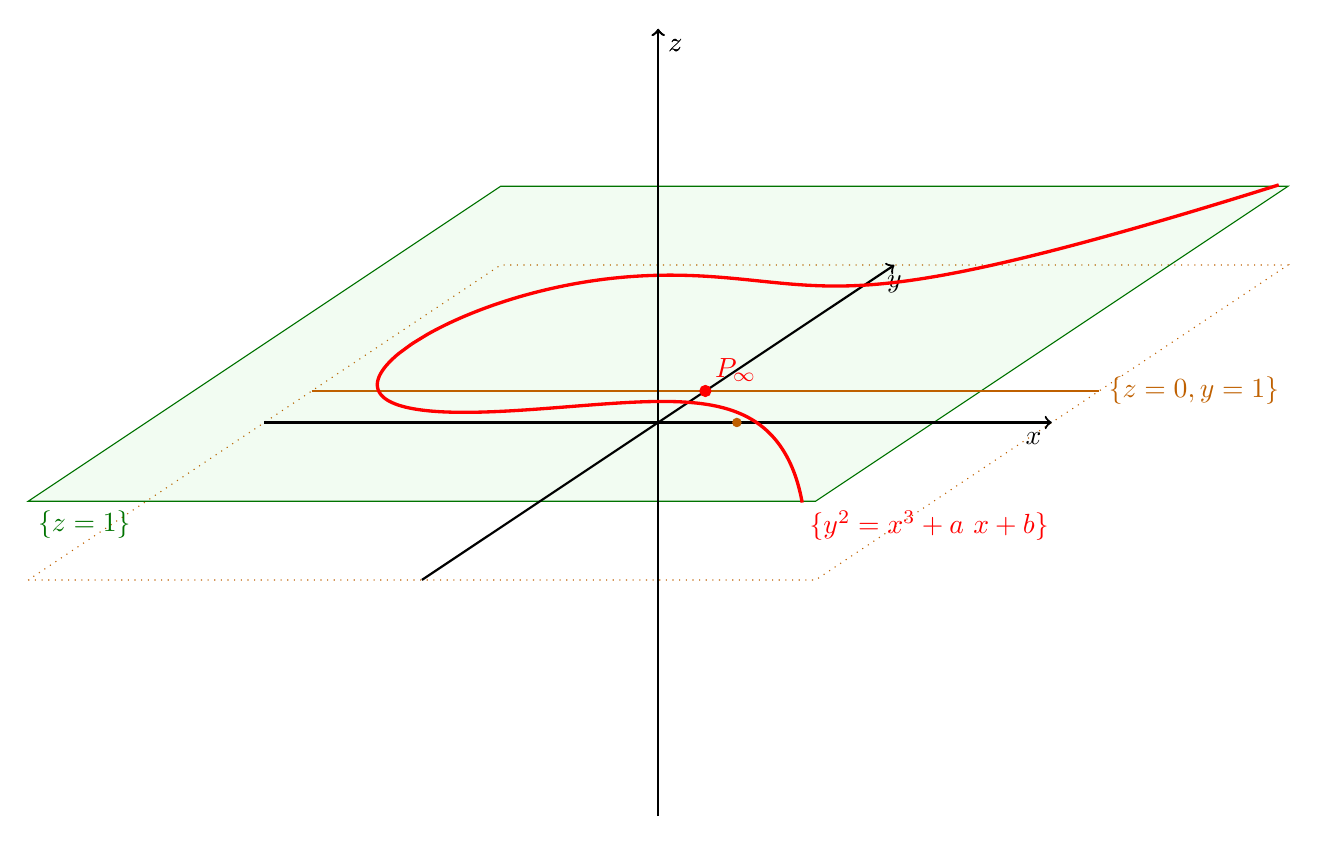
\begin{tikzpicture}[
		x={(1.0cm,0.0cm)},
		y={(0.6cm,0.4cm)},
		z={(0.0cm,1.0cm)}
	]

		% plane  z = 0
		\draw [orange!75!black, dotted] (-5,-5,0) -- (5,-5,0) -- (5,5,0) -- (-5,5,0) -- cycle;


		% plane z = 1
		\draw [green!45!black, fill = green!75!black, fill opacity = 0.05] (-5,-5,1) -- (5,-5,1) -- (5,5,1) -- (-5,5,1) -- cycle;
		\draw (-5,-5,1) node[green!45!black, anchor=north west]{$\{z = 1\}$};

		% line z = 0, y = 1
		\draw [thick, orange!75!black] (-5,1,0) -- (5,1,0);
		\draw (5,1,0) node[orange!75!black, anchor=west]{$\{z = 0, y = 1\}$};

		% axis
		\draw[thick,->] (-5,0,0) -- (5,0,0) node[anchor=north east]{$x$};;
		\draw[thick,->] (0,-5,0) -- (0,5,0) node[anchor=north]{$y$};;
		\draw[thick,->] (0,0,-5) -- (0,0,5) node[anchor=north west]{$z$};;

		\draw [orange!75!black, fill = orange!75!black] (1,0,0) circle[radius=1.5pt];

		% \draw [black, fill = black] (0,0,1) circle[radius=1.5pt];
		% \draw (0,0,1) node[anchor=south east]{$z = 1$};

		% Curve
		\draw[very thick,domain=-3.1243:4.86,smooth,variable=\x,red,samples=500] plot ({\x},{sqrt(0.45*0.5*\x*\x*\x - 0.45*2*\x + 0.45*9)},1);
		\draw[very thick,domain=-3.1243:4.86,smooth,variable=\x,red,samples=500] plot ({\x},{-sqrt(0.45*0.5*\x*\x*\x - 0.45*2*\x + 0.45*9)},1);
		\draw[very thick,red] (-3.1243,-0.02,1) -- (-3.1243,0.02,1);

		% P inf
		\draw [red, fill = red] (0,1,0) circle[radius=2pt];

		% equation
		\draw (4.8,-5,1) node[red, anchor=north west]{$\{y^2 = x^3 + a\ x + b\}$};
		\draw (0,1,0) node[red, anchor=south west]{$P_\infty$};

		\draw[thick,->] (0,0,1) -- (0,0,5) node[anchor=north west]{$z$};;

	\end{tikzpicture}

\end{document}
